\documentclass[
  bibliography=totoc,     % Literatur im Inhaltsverzeichnis
  captions=tableheading,  % Tabellenüberschriften
  titlepage=firstiscover, % Titelseite ist Deckblatt
]{scrartcl}

% Paket float verbessern
\usepackage{scrhack}

% Warnung, falls nochmal kompiliert werden muss
\usepackage[aux]{rerunfilecheck}

% deutsche Spracheinstellungen
\usepackage{polyglossia}
\setmainlanguage{german}

% unverzichtbare Mathe-Befehle
\usepackage{amsmath}
% viele Mathe-Symbole
\usepackage{amssymb}
% Erweiterungen für amsmath
\usepackage{mathtools}

% Fonteinstellungen
\usepackage{fontspec}
% Latin Modern Fonts werden automatisch geladen

\usepackage[
  math-style=ISO,    % ┐
  bold-style=ISO,    % │
  sans-style=italic, % │ ISO-Standard folgen
  nabla=upright,     % │
  partial=upright,   % ┘
  warnings-off={           % ┐
    mathtools-colon,       % │ unnötige Warnungen ausschalten
    mathtools-overbracket, % │
  },                       % ┘
]{unicode-math}

% traditionelle Fonts für Mathematik
\setmathfont{Latin Modern Math}
\setmathfont{XITS Math}[range={scr, bfscr}]
\setmathfont{XITS Math}[range={cal, bfcal}, StylisticSet=1]

% Zahlen und Einheiten
\usepackage[
  locale=DE,                 % deutsche Einstellungen
  separate-uncertainty=true, % immer Fehler mit \pm
  per-mode=reciprocal,       % ^-1 für inverse Einheiten
  output-decimal-marker={,},   % . statt , für Dezimalzahlen
]{siunitx}
\sisetup{math-micro=\text{µ},text-micro=µ}


% chemische Formeln
\usepackage[
  version=4,
  math-greek=default, % ┐ mit unicode-math zusammenarbeiten
  text-greek=default, % ┘
]{mhchem}

% richtige Anführungszeichen
\usepackage[autostyle]{csquotes}

% schöne Brüche im Text
\usepackage{xfrac}

% Standardplatzierung für Floats einstellen
\usepackage{float}
\floatplacement{figure}{htbp}
\floatplacement{table}{htbp}

% Floats innerhalb einer Section halten
\usepackage[
  section, % Floats innerhalb der Section halten
  below,   % unterhalb der Section aber auf der selben Seite ist ok
]{placeins}

%Floats innerhalb einer Subsection halten
\makeatletter
\AtBeginDocument{%
  \expandafter\renewcommand\expandafter\subsection\expandafter{%
    \expandafter\@fb@secFB\subsection
  }%
}
\makeatother

% Seite drehen für breite Tabellen
\usepackage{pdflscape}

% Captions schöner machen.
\usepackage[
  labelfont=bf,        % Tabelle x: Abbildung y: ist jetzt fett
  font=small,          % Schrift etwas kleiner als Dokument
  width=0.9\textwidth, % maximale Breite einer Caption schmaler
]{caption}
% subfigure, subtable, subref
\usepackage{subcaption}

% Grafiken können eingebunden werden
\usepackage{graphicx}
% größere Variation von Dateinamen möglich
\usepackage{grffile}

% schöne Tabellen
\usepackage{booktabs}

% Verbesserungen am Schriftbild
\usepackage{microtype}

% Literaturverzeichnis
\usepackage[
  backend=biber,
]{biblatex}
% Quellendatenbank
\addbibresource{lit.bib}
\addbibresource{programme.bib}

% Hyperlinks im Dokument
\usepackage[
  unicode,        % Unicode in PDF-Attributen erlauben
  pdfusetitle,    % Titel, Autoren und Datum als PDF-Attribute
  pdfcreator={},  % ┐ PDF-Attribute säubern
  pdfproducer={}, % ┘
]{hyperref}
% erweiterte Bookmarks im PDF
\usepackage{bookmark}

% Trennung von Wörtern mit Strichen
\usepackage[shortcuts]{extdash}

%keine Einrückung am Anfang des Absatzes
%\parindent 0pt

\author{
  Timo Gräßer
  \texorpdfstring{
    \\
    \href{mailto:timo.graesser@udo.edu}{timo.graesser@udo.edu}
  }{}%
  \texorpdfstring{\and}{, }
  Jasper Karl Lammering%
  \texorpdfstring{
    \\
    \href{mailto:jasper.lammering@udo.edu}{jasper.lammering@udo.edu}
  }{}%
}
\publishers{TU Dortmund – Fakultät Physik}

%eigener Befehl
%symup
\newcommand*\dif{\mathop{}\!\mathrm{d}}
\ExplSyntaxOn
\NewDocumentCommand \g {m}
 {
  \ensuremath{
    \symup{#1}
  }
 }


\NewDocumentCommand \pdif {mmo}{
    \IfNoValueTF {#3} {
         \frac{\partial #1}{\partial #2}
    }{
         \left(\frac{\partial #1}{\partial #2}\right)\sb{#3}
    }
}

\NewDocumentCommand \tdif {mm}{\frac{\dif #1}{\dif #2}}

\NewDocumentCommand{\underarrow}{mm}{
  \underset{\makebox[0pt]{\begin{tabular}{@{}c@{}}\ensuremath{\uparrow}\\[0pt] $\small #2$ \end{tabular}}}{#1}
}

\ExplSyntaxOff
\DeclareMathOperator{\e}{e}


\subject{V 59}
\title{Modulation und Demodulation elektrischer Schwingungen}
\date{
  Durchführung: 16.04.2018
  \hspace{3em}
  Abgabe: 24.04.2018
}

\begin{document}

\maketitle
\thispagestyle{empty}
\tableofcontents
\newpage

\section{Theorie}
\label{sec:Theorie}

\subsection{Fehlerrechnung}

Für die Fehlerfortpflanzung bei Gleichungen mit $N$ fehlerbehafteten Größen
wird jeweils die Formel zur Gaußschen Fehlerfortpflanzung

\begin{equation*}
  \sigma = \sqrt{\sum_{i=1}^{N}\biggl(\frac{\partial f(x_{\g{i}})}{\partial x_{\g{i}}}
  \sigma_{\g{i}}\biggr)^2}
\end{equation*}
mit der jeweiligen Funktion $f(x_{\g{i}})$, den Messgrößen $x_{\g{i}}$ und den
zugehörigen Fehlern $\sigma_i$ verwendet.
Zur Berechnung des arithmetischen Mittels von $N$ Messwerten wird jeweils die
Formel

\begin{equation*}
  \overline{x} = \frac{1}{N}\sum_{i=1}^{N}x_{\g{i}}
\end{equation*}
mit den Messwerten $x_i$ benutzt.
Die Standardabweichung des Mittelwerts wird jeweils mit der Gleichung

\begin{equation*}
  \overline{\sigma} = \sqrt{\frac{1}{N-1}\sum_{i=1}^{N}(x_{\g{i}} - \overline{x})^2}
\end{equation*}
mit den $N$ Messwerten $x_i$ berechnet.

\subsection{Einleitung}

Auf mikroskopischer Skala sind die Ladungsdichte $\rho$ und die Stromdichte $\vec{j}$ in einem Leiter
schwankende Größen. Das ist darin begründet, dass die Elementaradung diskontiniuerlich ist und somit nicht den
ganzen Raum gleichmäßig füllt und sich außerdem die Ladungsträger ungeordnet bewegen. Dies hat zur Folge, dass
mit empfindlichen Messgeräten statistische Schwankungen, das sogenannte Rauschen, in der Spannung $U$ und der
Stromstärke $I$ in einem Schaltkreis detektierbar sind. Im Folgenden werden unterschiedliche Formen
des Rauschens vorgestellt und im Anschluss daran experimentell untersucht.

\subsection{Verschiedene Rauschphänomene}

Unter dem thermischen Rauschen versteht man das Spannungsrauschen an einem ohmschen Widerstand. Durch
ungeordnete Bewegung der Elektronen bei endlicher Temperatur entstehen stellenweise Ladungsüberschüsse
und dadurch messbare Potentialdifferenzen. Ein typischer Spannungsverlauf ist in Abbildung \ref{fig:thermtyp}
skizziert.

\begin{figure}
  \centering
  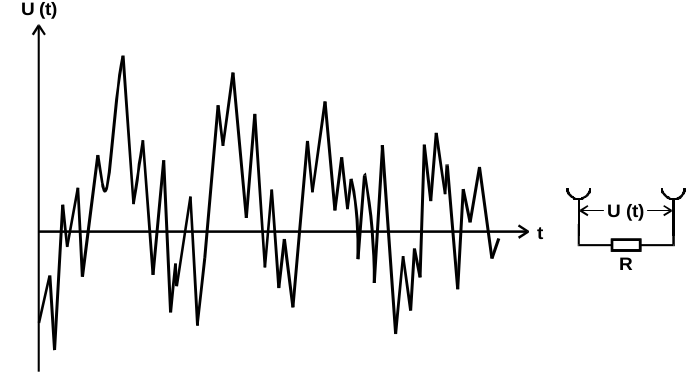
\includegraphics[height=5cm]{Dickpics/thermtyp.png}
  \caption{Ein typischer Spannungsverlauf, der an den Enden eines ohmschen Widerstandes bobachtet werden kann \cite{fig:thermtyp}.}
  \label{fig:thermtyp}
\end{figure}

Das sogenannte Stromrauschen tritt beispielsweise auf, wenn Elektronen aus Festkörperoberflächen emittiert werden.
Dabei wird zwischen zwei Effekten, die für das Rauschen verantwortlich sind, unterschieden.

In einer Diode beispielsweise entsteht ein Stromrauschen, da die an der Kathode emittierten Elektronen in unregelmäßigen Abständen
auf die Anode treffen. Die Abweichungen in der Stromstärke sind zwar klein, können aber mit geeigneten Messgeräten
sichtbar gemacht werden. Das unregelmäßige Auftreffen der Elektronen auf die Anode ist vergleichbar mit dem Auftreffen von Schrotkörnern
auf eine Metallplatte, weshalb dieses Phänomen Schrot-Effekt genannt wird.

Der Funkel-Effekt beschreibt ein Stromrauschen, welches entsteht, wenn die Austrittsarbeit an der Kathode zeitabhängig ist.
Dies spielt vor allem bei Oxydkathoden eine große Rolle und soll in diesem Versuch ebenso wie der Schroteffekt untersucht
werden.

\subsection{Stationäre und Ergodische Schwankungserscheinungen}

Um einen Rauschprozess zu quantifizieren ist es nicht zweckmäßig den genauen Verlauf
von Schwankungen zu untersuchen, da zumindest die im vorangegangenen Abschnitt vorgestellten
Rauschphänomene stochastische, zum Teil indeterministische, Prozesse sind. Stattdessen
werden geeignete Mittelwerte von Rauschströmen bzw. -spannungen untersucht.
Der zeitliche Mittelwert einer Rauschspannung verschwindet i.A., wenn diverse Parameter, zum Beispiel
die Temperatur, konstant gehalten werden. Der quadratische Mittelwert
\begin{align}
  \overline{U^2}(\tau) = \frac1{\tau} \int_{0}^{\tau} U^2(t) \mathrm{d}t
\end{align}
hingegen ist i.A. nicht Null und beinhaltet Informationen über den Rauschprozess im Zeitintervall $[0,\tau]$. Wenn dieser Wert
unabhängig von der Wahl des Zeitintervalls ist, also alle Parameter, die Einfluss auf das Rauschen haben, konstant
gehalten werden, wird die Schwankungserscheinung als stationär bezeichnet.
Das sogenannte Scharmittel
\begin{align}
  \langle U^2(t_0) \rangle = \frac1{N} \sum_{i=1}^{N} U_i^2(t_0)
\end{align}
ergibt sich über Mittelung mehrerer identischer Rauschquellen zum selben Zeitpunkt $t_0$.
Sind Scharmittel und Zeitmittel gleich, so wird die Schwankungserscheinung als ergodisch bezeichnet.
Das ist zum Beispiel beim thermischen Widerstandsrauschen oder beim Schroteffekt der Fall, wenn sämtliche
Parameter wie die Temperatur oder der mittlere Diodenstrom konstant gehalten werden.

Da die vorgestellten Schwankungserscheinungen, wie bereits erwähnt, mikroskopischer Natur sind,
lassen sich mittels verschiedener Messungen mikroskopische Größen bestimmen. So soll in diesem
Versuch die Elementarladung $\mathrm{e}_0$ und die Boltzmannsche Konstante $k_\text{B}$ experimentell durch eine
Rauschmessung bestimmt werden. Dazu werden zunächst theoretische Zusammenhänge für die erwähnten Rauschprozesse hergeleitet.

\subsection{Das Thermische Rauschen und die Nyquist-Beziehung}

Aus einem Gedankenexperiment einer verlustosen Doppelleitung, die durch zwei Widerstände
kurzgeschlossen wird, und diverser Annahmen aus der statistischen Thermodynamik kann eine
Beziehung zwischen dem quadratischen Rauschspannungsmittelwert $\overline{U^2}$ und der Temperatur
$T$ hergeleitet werden. Diese sogenannte Nyquist-Beziehung lautet
\begin{align}
  \overline{U^2} = 4 k_\text{B} \cdot T \cdot R \cdot \Delta \nu.
\end{align}
Dabei ist $R$ der Widerstand der Rauschquelle und $\Delta \nu$ das Frequenzintervall der Rauschspannung. Da
$\overline{U^2}$ nicht dispersiv ist, sondern nur von der Breite des Frequenzintervalls abhängig ist, wird das Rauschen des Widerstands auch weißes Rauschen genannt.
Es ist zu beachten, dass diese Gleichung nur in einem Frequenzbereich von unter $\SI{6e11}{\hertz}$ gilt,
wie in Abbildung \ref{fig:freqab} dargestellt, darüber ist $\overline{U^2}$ dispersiv. Bei Zimmertemperatur gilt jedoch die Relation
$h\nu \ll k_\text{B}T$ und damit auch die Nyquist-Beziehung.

\begin{figure}
  \centering
  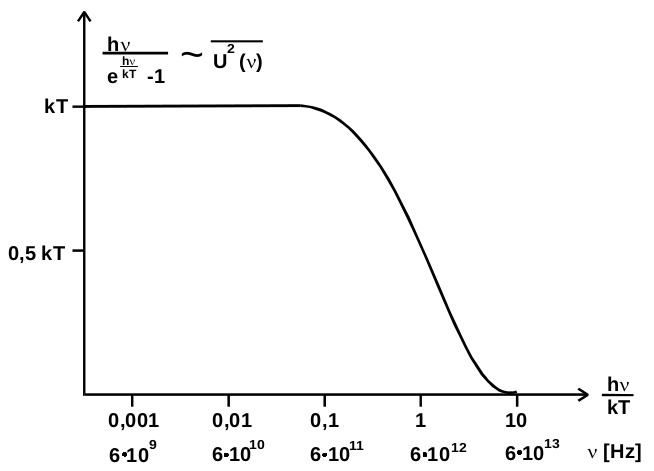
\includegraphics[height=7cm]{Dickpics/freqab.png}
  \caption{Frequenzabhängigkeit des quadratischen Rauschspannungsmittelwerts beim thermischen Widerstandsrauschen \cite{anleitung}.}
  \label{fig:freqab}
\end{figure}

Des Weiteren muss beachtet werden, dass ein realer Widerstand immer eine endliche Eigenkapazität besitzt. Das Ersatzschaltbild
dazu ist in Abbildung \ref{fig:ersatzschaltbildR} zu sehen. Über die Maschenregel folgt das effektive, messbare Spannungsrauschen
\begin{align}
  \overline{U_{\text{RC}}^2} = \overline{U_{\text{R}}^2} \cdot \frac1{1+(2\pi\nu_\text{m} RC)^2},
\end{align}
wobei $\nu_\text{m}$ hier der Mittelwert des betrachteten Frequenzintervalls $\Delta \nu$ ist.

\begin{figure}
  \centering
  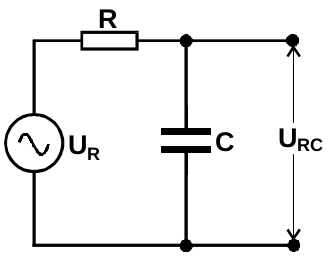
\includegraphics[height=3.7cm]{Dickpics/ersatzschaltbildR.png}
  \caption{Ersatzschaltbild des realen Widerstandes mit einem idealen ohmschen Widerstand $R$ und einer idealen Kapazität $C$ \cite{anleitung}.}
  \label{fig:ersatzschaltbildR}
\end{figure}

\subsection{Das Schrotrauschen und die Schottky-Beziehung}

Zur Messung des Schrotrauschens einer Reinmetallkathode eignet sich die in Abbildung \ref{fig:schrotdiode} skizzierte
Versuchsanordnung. Die Anodenspannung sollte dabei so hoch gewählt sein, dass die Diode im Sättigungsbereich arbeitet,
damit alle an der Kathode emittierten Elektronen die Anode erreichen.
Der gesamte Anodenstrom lässt sich aufspalten in
\begin{align}
  I_\text{ges}(t) = I_0 + I(t),
\end{align}
wobei $I_0$ der mittlere Anoden(gleich)strom und $I(t)$ der Rauschstrom ist, dessen Mittelwert Null ist.
Um eine Beziehung für das mittlere Rauschstromquadrat $\overline{I^2}$ herzuleiten, werden
folgende Annahmen gemacht:
\begin{enumerate}%[(a)]
  \item Die Elektronen werden unabhängig voneinander an der Kathode emittiert.
  \item Die Bewegung der Elektronen auf dem Weg zu Anode wird nicht durch andere Elektronen
  beeinflusst und ist bei allen Elektronen annähernd äquivalent. \\
  $\to$ Sättigungsbereich
  \item Die Elektronen starten mit $v \approx 0$.
  \item Es entstehen keine Sekundärelektronen an der Anode.
\end{enumerate}

\begin{figure}
  \centering
  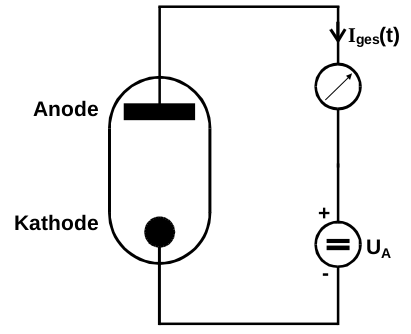
\includegraphics[height=5cm]{Dickpics/schrotdiode.png}
  \caption{Schaltbild der Reinmetalldiode zur Ausmessung des Schrotrauschens \cite{anleitung}.}
  \label{fig:schrotdiode}
\end{figure}

Das zum Zeitpunkt $t_n$ emittierte Elektron induziert durch Influenzwirkung einen Strom
\begin{align}
  I_n(t) = \mathrm{e_0} f(t-t_n)
\end{align}
in der Anode. Die Funktion $f(t-t_n)$ beschreibt dabei die Form des Stromimpulses und ist nur
im Flugzeitintervall $\tau$ von Null verschieden. Der gesamte Anodenstrom ergibt sich durch Summation
gemäß
\begin{align}
  I_\text{ges}(t) = \mathrm{e}_0 \sum_n f(t - t_n).
\end{align}
Durch Ausnutzen des Campbellschen Theorems und der Parsevalidentität folgt die spektrale Verteilungsfunktion des Schrotrauschens
\begin{align}
  W_\text{Schrot}(\nu) = 2 \mathrm{e}_0 I_0 \left| F(\nu) \right|^2.
\end{align}
Dabei ist $F(\nu)$ die Fouriertransformierte eines Einzelstromimpulses $f(t)$.
Im Niederfrequenzbereich
\begin{align}
  \nu \ll \frac1{2\pi\tau},
\end{align}
also wenn die Emissionsperiodendauer der Elektronen wesentlich größer als die Flugzeit $\tau \approx \SI{3}{\nano\second}$ der Elektronen ist, gilt
\begin{align}
  F(\nu) \approx 1.
\end{align}
Insgesamt ergibt sich in diesem Bereich
\begin{align}
  \overline{I^2} = 2 \mathrm{e}_0 I_0 \Delta \nu.
\end{align}
Diese Relation wird auch Schottky-Beziehung genannt und stellt ebenfalls ein weißes Rauschen dar,
da $\overline{I^2}$ nicht dispersiv ist. Die Voraussetzungen 3. und 4. sind im betrachteten
Niederfrequenzbereich nicht relevant, da spürbare Effekte durch endliche Anfangsgeschwindigkeiten
und Sekundärelektronen erst bei Frequenzen im ausgeschlossenen Bereich $\nu \approx 1/2\pi\tau$ auftreten.
Es ist jedoch essentiel wichtig, dass die Diode im Sättigungsbereich betrieben wird.
Ansonsten wird das Rauschen effektiv abgeschwächt, da dichter bzw. weniger dicht beieinander
emittierte Elektronen eine Raumladung erzeugen, die der Dichteschwankung entgegenwirkt. Es ist daher
zu erwarten, dass $\overline{I^2}$ in diesem Bereich kleiner als durch die Schottky-Beziehung vorausgesagt ist.

\subsection{1/f-Rauschen und der Funkel-Effekt}

Durch Generations-Rekombinations-Prozesse von Ladungsträgern in Oxid-Halbleiter-Grenzschichten entstehen
Rauschströme, deren spektrale Leistungsdichte in bestimmten Frequenzbereichen proportional zur reziproken Frequenz ist.
Allgemein lässt sich herleiten, dass die spektrale Leistungsdichte für das sogenannte Generations-Rekombinations-Rauschen
\begin{align}
  W_\tau(\nu) = \text{const} \frac{\tau}{1+(2 \pi \nu \tau)^2}
\end{align}
ist, wobei $\tau$ die Relaxationszeitkonstante für einen Generations-Rekombinations-Prozess ist.
Für $\nu \ll 1/\tau$ ist $W_\tau(\nu)$ nicht dispersiv, es liegt also weißes Rauschen vor.
Sobald $\nu \propto 1/\tau$ fällt die spektrale Leistungsdichte ab, wie auch den gestrichelten Linien
in Abbildung \ref{fig:leistungsdichte} entnehmbar ist. Wenn die Relaxationszeit variabel ist, wie es in der
Realität auch der Fall ist, dann ist dieser Abfall der Leistungsdichte proportional zur reziproken Frequenz
und es liegt ein 1/f-Rauschen vor.

\begin{figure}
  \centering
  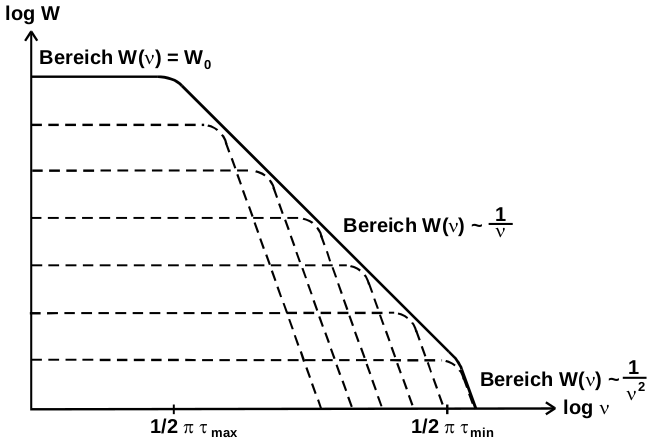
\includegraphics[height=6.5cm]{Dickpics/leistungsdichte.png}
  \caption{Schematischer Verlauf der spektralen Leistungsdichte beim Generations-Rekombinations-Rauschen. Die gestrichelten Linien
  beschreiben den Verlauf bei fester Relaxationszeit $\tau$. Liegt $\tau$ variabel in einem Intervall $[\tau_\text{min}, \tau_\text{max}]$
  so ergibt sich ein 1/f-Rauschen, hier dargestellt durch die durchgezogene Linie \cite{anleitung}.}
  \label{fig:leistungsdichte}
\end{figure}

Nimmt man für die Relaxationszeit $\tau$ einen exponentiellen Zusammenhang
\begin{align}
  \tau(E) = \tau_0 \text{exp}\left(\frac{E}{k_\text{B}T}\right)
\end{align}
zur Aktivierungsenergie $E$ eines Generations-Rekombinations-Prozesses an, so ergibt sich die spektrale Leistungsdichte
\begin{align}
  W(\nu) = \frac{\text{const} k_\text{B} T}{\nu} \left\{ \arctan{(2\pi\nu\tau_\text{min})} - \arctan{(2\pi\nu\tau_\text{max})} \right\}.
\end{align}
Die Werte $\tau_\text{min}$ bzw. $\tau_\text{max}$ beschränken die Relaxationszeit auf ein Intervall, wie auch
die Aktivierungsenergie auf ein Intervall $[E_\text{min}, E_\text{max}]$ beschränkt ist.
Es können nun anhand der Grenzfälle
\begin{align}
  \arctan{(x)} &\to x \qquad \, \text{für} &x &\to 0 \\
  \arctan{(x)} &\to \frac{\pi}{2} \qquad \text{für} &x &\to \infty
\end{align}
qualitativ drei Frequenzbereiche unterschieden werden:
\begin{enumerate}
  \item Für $2\pi\nu\tau \ll 1$ resultiert keine Frequenzabhängigkeit und daher weißes Rauschen.
  \item Für $2\pi\nu\tau_\text{min} \ll 1$ und $2\pi\nu\tau_\text{max} \gg 1$ resultiert
  \begin{align}
    W(\nu) = \frac{\text{const} k_\text{B} T}{\nu} \frac{\pi}{2}
  \end{align}
  und daher 1/f-Rauschen.
  \item Für $2\pi\nu\tau \gg 1$ resultiert eine $1/\nu^2$-Abhängigkeit.
\end{enumerate}
Ein 1/f-Rauschen entsteht beispielsweise an einer Oxid-Metall-Kathode durch eine sich zeitlich ändernde Austrittsarbeit,
was wie bereits erwähnt als Funkel-Effekt bezeichnet wird. Dieses Rauschen überlagert sich mit dem weißen Schrotrauschen, das
im vorangegangenen Kapitel behandelt wurde.
Abhängig vom Diodenstrommittelwert $I_0$ ergibt sich für das Frequenzspektrum des Rauschens durch den Funkeleffekt
\begin{align}
  W_\text{Funkel}(\nu) = \frac{\text{const} I_0^2}{\nu^\alpha},
\end{align}
wobei $\alpha \approx 1$.

\subsection{Versuchsaufbauten zur Ausmessung des thermischen Widerstandsrauschen}

In Abbildung \ref{fig:rauschspektro} ist das Blockschaltbild eines einfachen Rauschspektrometers skizziert.

\begin{figure}
  \centering
  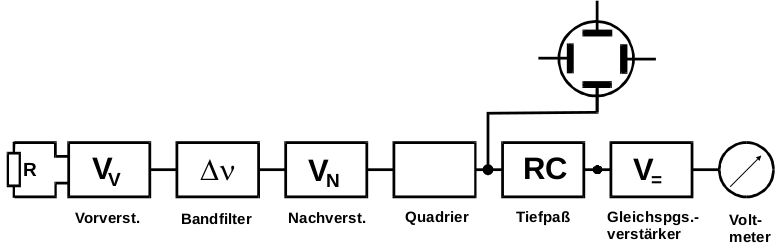
\includegraphics[height=4cm]{Dickpics/rauschspektro.png}
  \caption{Blockschaltbild eines einfachen Rauschspektrometers \cite{anleitung}.}
  \label{fig:rauschspektro}
\end{figure}

Die Amplituden der Rauschspannungssignale am Widerstand $R$ werden zunächst im Vorverstärker mit dem Faktor $V_\text{V}$ linear verstärkt
und daraufhin am Bandfilter diejenigen Frequenzen herausgefiltert, die außerhalb des Frequenzintervalls $\Delta \nu$ liegen.
Die übrigen Signale werden im Nachverstärker um den Faktor $V_\text{N}$ nachverstärkt und an einen Quadrierer weitergegeben,
welcher aus den eintreffenden Spannungssignalen das Signal $V_\text{V}^2 V_\text{N}^2 U_R^2(t)$ bildet. Dieses läuft anschließend
in einen Tiefpass, wo der Gleichspannungsanteil herausgefiltert wird, und kann, nachdem es in einem Gleichspannungsvertärker
mit $V_=$ verstärkt wird, am Voltmeter gemessen werden. Im Idealfall wird also die Größe
\begin{align}
  U_\text{A}^2 = V_= V_\text{V}^2 V_\text{N}^2 \overline{U_R^2} = V_= V_\text{V}^2 V_\text{N}^2 \Delta \nu 4 k_\text{B} T R
  \label{eqn:Uarauschspektro}
\end{align}
gemessen. Dabei ist $V_\text{V}^2 V_\text{N}^2 \Delta \nu$ eine Apparaturkonstante, die durch eine Eichmessung bestimmt werden kann, sodass
zuletzt die Boltzmannkonstante $k_\text{B}$ bestimmt werden kann. Gleichung \eqref{eqn:Uarauschspektro} gilt jedoch nur im Falle
idealer Apparaturen. In der Realität produzieren alle Bauteile Rauschspannungen, die sich mit der des Widerstands überlagern und das
Ergebnis verfälschen. Das fällt vor allem beim Vorverstärker ins Gewicht, da dessen Eigenrauschen insgesamt am stärksten nachverstärkt wird.
Indem ein Nullwiderstand, anstatt des ohmschen Widerstandes $R$ am Eingang des Rauschspektrometers angeschlossen wird, kann eine Abschätzung
des Apparatureigenrauschens gemacht werden und falls nötig Messwerte um einen Offset korrigiert werden.
Dazu ist ein Ersatzschaldbild für einen Verstärker mit Eigenrauschen in Abbildung \ref{fig:verstärkerrauschen} dargestellt.

\begin{figure}
  \centering
  \includegraphics[height=5cm]{Dickpics/verstärkerrauschen}
  \caption{Ersatzschaltbild eines Verstärkers mit Eigenrauschen \cite{anleitung}.}
  \label{fig:verstärkerrauschen}
\end{figure}

Nimmt man gemäß der Abbildung die Spannung
\begin{align}
  U_1(t) = U_R(t) + U(t) + I(t)
\end{align}
am Eingang des Vorverstärkers an, so ergibt sich am Ausgang des Rauschspektrometers
\begin{align}
  U_\text{A}^2 = V_\text{ges}^2 \overline{U_R^2} + V_\text{ges}^2 \left( R^2 \overline{I^2} + 2 R \overline{U I} + \overline{U^2} \right) \approx V_\text{ges}^2 \overline{U_R^2} + V_\text{ges}^2 \overline{U^2},
\end{align}
wobei die Näherung für die im Versuch vorliegenden Vorverstärker mit MOS-Feldeffekttransistoren gerechtfertigt ist.
Die Messung des Verstärkerrauschterms $V_\text{ges}^2 \overline{U^2}$ erfolgt, wie bereits erwähnt, durch Kurzschließen des
Rauschspektrometereingangs.

Für Verstärkerrauschspannungen $|U| \gg |U_R|$ wird das im vorangegangenen Teil beschriebene Verfahren ungenau und es eignet sich
anstatt dessen die in Abbildung \ref{fig:korrelatorschaltung} dargestellte, sogenannte Korrelatorschaltung.

\begin{figure}
  \centering
  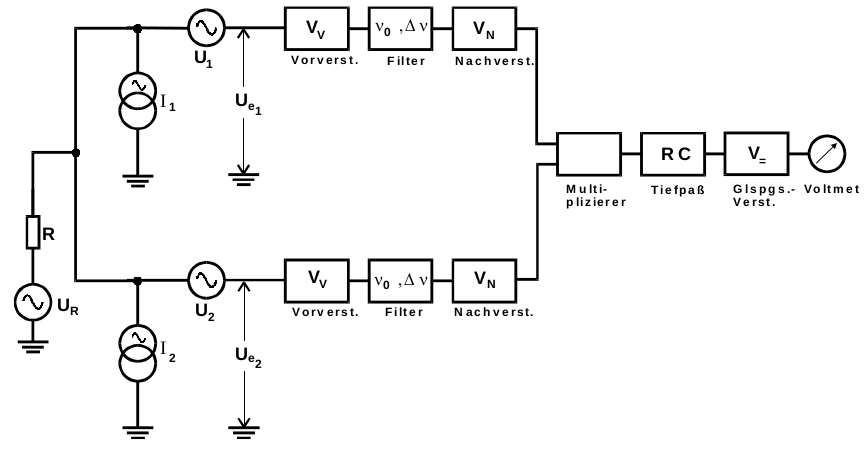
\includegraphics[height=7.3cm]{Dickpics/korrelatorschaltung.png}
  \caption{Blockschaltbild der Korrelatorschaltung zur Ausmessung des thermischen Widerstandsrauschens \cite{anleitung}.}
  \label{fig:korrelatorschaltung}
\end{figure}

Bei dieser Schaltung ergibt sich die Ausgangsspannung zu
\begin{align}
  U_\text{A,korr}^2 = V_\text{ges}^2 \left \{ \overline{U_R^2} + R \left( \overline{U_1 I_1} + \overline{U_2 I_2} \right) + R^2 \left( \overline{I_1^2} + \overline{I_2^2} \right) \right \} \approx V_\text{ges}^2 \overline{U_R^2},
\end{align}
sofern erneut Vorverstärker mit MOS-Feldeffekttransistoren verwendet werden. Das Verstärkerrauschen ist also näherungsweise Null, obwohl
mit dieser Schaltung dieselbe Verstärkung erreicht werden kann.

Mit Hilfe der Rauschzahl
\begin{align}
  F(\nu_0,Z) = \frac{\overline{U_\text{A}^2}(Z)}{4 k_\text{B} T \Delta \nu V_\text{ges}^2 \cdot \text{Re}(Z)}
\end{align}
können Aussagen über das Eigenrauschen und damit über die Qualität eines Verstärkers abhängig von der
Lage $\nu_0$ des Durchlassbereichs und dem Wellenwiderstand $Z$ des angeschlossenen Rauschelements gemacht werden.
Der niedrigste und gleichzeitig optimalste Wert für die Rauschzahl ist $F = 1$.




\cite{anleitung}

 \section{Durchführung}
\label{sec:Durchführung}
\subsection{Aufbau}
\begin{figure}
  \centering
  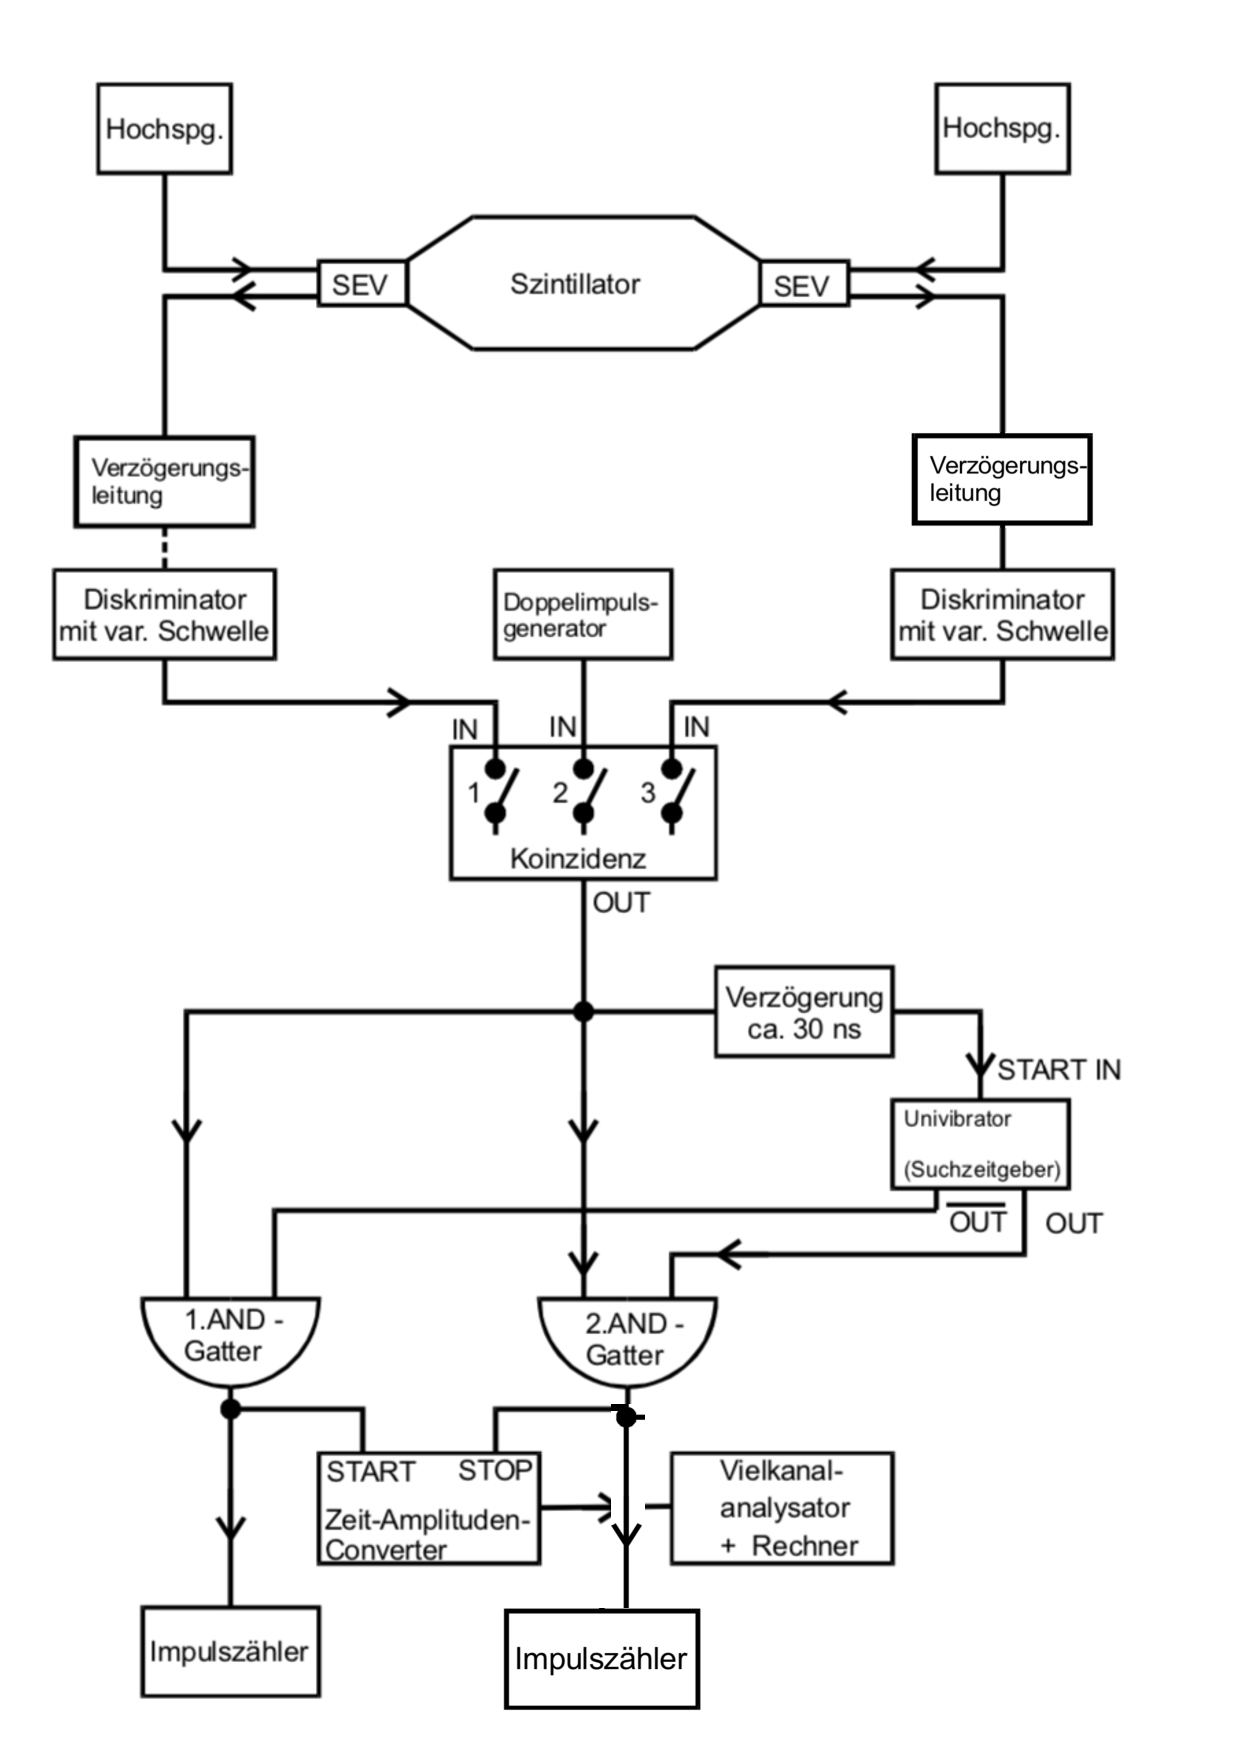
\includegraphics[width=\textwidth]{leuteBeimKacken/Schaltung.pdf}
  \caption{Blockschaltbild der hier genutzten Schaltung.\cite{anleitung}}
  \label{fig:Schaltung}
\end{figure}

In Abbildung \ref{fig:Schaltung} wird die Schaltung gezeigt. Im Folgenden werden die einzelnen Bestandteile von oben nach unten kurz beschrieben.

Der zentrale Detektor ist ein \SI{50}{\litre} großer Szintillationstank. Wie oben beschrieben ist er mit organischem Szintillator gefüllt. Diese haben im Allgemeinen eine kürzere Ansprechzeit als anorganische. Zur Aufnahme der darin erzeugten Lichtsignale und zur Übersetzung in elektrische Spannungsimpulse sind an den Enden des Tanks Photomultiplier angebracht. Diese können auch durch thermisches Rauschen ein Signal erzeugen. Um dessen Einfluss auf die Messung zu reduzieren wird eine Koinzidenzschaltung aufgebaut, die also nur ein Signal liefert, wenn in beiden SEVs gleichzeitig ein Signal auftritt. Dieses Verfahren funktioniert, weil das Rauschen der beiden SEVs unkorreliert verläuft und deshalb nur ein Myonsignal gleichzeitig in beiden SEVs ein Signal erzeugt. Ein Ausgleich der systematischen elektronischen relativen Verzögerung eines SEVs zum anderen wird durch eine Verzögerungsleitung geleistet. Eine zusätzliche Rauschunterdrückung wird durch Diskriminatoren geleistet, die Signale bis zu einer einstellbaren Schwelle nicht durchlassen. Ein solcher Diskriminator liefert einen Normimpuls wenn diese Schwelle überschritten wird. Die Breite und Höhe dieses Pulses lassen sich einstellen.
Da Rauschpulse augrund ihrer Entstehung durch einzelne Elektronen kleiner als Signalpulse sind, werden sie reduziert.

Der Koinzidenzschaltung folgend befindet sich die Stoppuhrschaltung. Diese teilt das Signal zunächst auf je einen Eingang zweier logischer AND-Gatter sowie einen Univibrator auf. Diese drei Bauteile erhalten immer das Signal. Je nach zeitlichem Abstand zweier Signale, dem damit verbundenen Verhalten des Unvibrators und aufgrund der logischen Schaltung werden verschiedene Effekte ausgelöst.
Der Univibrator hat einen normalen und einen invertierten Ausgang. Bei eintreffendem Signal gibt zunächst der normale Ausgang das Signal weiter und der invertierte nicht. Dann startet die einstellbare Suchzeit. Ein Signal das innerhalb dieser Zeit eintrifft wird am invertierten Ausgang ausgegeben. Wenn die Zeit abgelaufen ist, ohne dass ein Signal eingetroffen ist, schaltet der Univibrator wieder auf den normalen Ausgang.
So bald nun ein Myonsignal in die Schaltung eintritt, erhält das erste AND-Gatter sowohl von der direkten Leitung als auch von der Leitung über den normalen Ausgang des Univibrators ein Signal.
Damit sendet es ein Signal weiter an den Start-Eingang des später beschriebenen Zeit-Amplituden-Converter (TAC).
% Nach Aussendung des Signals an das erste AND-Gatter startet im Univibrator die einstellbare Suchzeit $T_\text{S}$ nach einem zweites Signal. Ein Signal das innerhalb dieser Zeit den Univibrator durchquert wird nicht an das erste dafür aber an das zweite AND-Gatter weitergeleitet.
Wenn dann ein Signal innerhalb der Suchzeit des Unvibrators eintrifft, wird es vom invertierten Eingang ans zweite AND-Gatter geleitet.
Dieses erhält also dann an beiden Eingängen ein Signal und sendet so ein Signal an den Stopp-Eingang des TAC.
Diese Methode kann benutzt werden, da der mittlere zeitliche Abstand von zwei einfallenden Myonen klein gegenüber ihrer Lebensdauer ist. Ein über den gesamten Zerfallszeitbereich konstanter Untergrund hat seinen Ursprung also darin dass zwei Myonen statistisch bedingt mit einem zeitlichen Abstand von $t<T_\text{S}$ in den Tank eintreten. $T_\text{S}$ sollte also so groß gewählt werden, dass möglichst viele Messwerte der Zerfallszeiten genommen werden können, aber so klein, dass der Untergrund nicht zu groß wird.
Der TAC wandelt den zeitlichen Abstand von Start- und Stopp-Signal in einen dem proportional großen Spannungsimpuls um. Dieser wird an einen Vielkanalanalysator geleitet. Dort wird die Häufigkeit der Pulse ihrer Höhe entsprechend in Kanälen gezählt.
Das Histogramm der Kanäle kann im Rechner ausgelesen werden.

\subsection{Einstellen der Apparatur}
Um sich mit der Apparatur vertraut zu machen, sie aufzubauen und ihre Funktionsweise zu überprüfen werden vor der eigentlichen Messung einige Tests durchgeführt.

Zunächst werden die Impulse aus den SEVs vor und nach den Diskriminatoren am Oszilloskop untersucht. Vorher sollten sie unterschiedliche Eigenschaften besitzen und danach gleich hoch und lang sein. Dabei kann die Breite der Pulse eingestellt werden.
Diese sollte klein gegenüber der Lebensdauer der Myonen sein, damit sich zwei Impulse möglichst nicht überlagern.
Außerdem wird mit einem Zählwerk überprüft, ob beide Leitungen ähnliche Impulsraten aufweisen und dies mit der Schwelle am Diskriminator eingestellt. Darauf folgend wird untersucht welche Verzögerungszeit zwischen den SEVs die maximale Zählrate nach der Koinzidenzschaltung liefert. Dazu wird die Verzögerung in beide Richtungen variiert und für je zehn Sekunden die Impulszahl gemessen.
Außerdem wird die Zählrate nach der Koinzidenzschaltung mit den Zählraten der Eingänge verglichen um die Rauschunterdrückung zu überprüfen.

Als nächstes werden Univibrator und TAC justiert. Die Suchzeit des Univibrators wird etwas größer eingestellt als der Zeitmessbereich des TAC. Mit Hilfe eines Doppelimpulsgenerators wird überprüft ob der TAC korrekt arbeitet, also Spannungsimpulse liefert dessen Höhe proportional zum zeitlichen Abstand der Impulse ist. Dies wird am PC mit Vielkanalanalysator kontrollliert. So wird auch eine Zeitkalibrierung durchgeführt, da man den eingestellten Abstand der Impulse so einem Kanal zuordnen kann.

Um abzuschätzen wie oft Myonen detektiert werden, also auch die die nicht im Behälter zerfallen, wird noch an das erste AND-Gatter ein Zählwerk angeschlossen. Außerdem wird am zweiten AND-Gatter ein Impulszähler angeschlossen um einen Wert für die Anzahl an gemessenen Zerfallszeiten zu erhalten. Mit diesen Werten kann zusammen mit der Messzeit der Untergrund bestimmt werden.

Dann kann mit der eigentlichen Messung begonnen werden, bei der die individuellen Lebensdauern \num{20} bis \num{30} Stunden aufgenommen werden und als Histogramm dargestellt werden. Dann kann mit der in Kapitel \ref{sec:Lebensdauerbestimmung} beschriebenen Methode die mittlere Lebensdauer bestimmt werden.

\section{Results}
\label{sec:Auswertung}

\subsection{Laser Mode}

As the first step we determine the current treshold from which on the diode is in laser mode. To get a visual indication of the transition from LED to laser diode a IR viewing card is placed in front of the laser. This card emitts light in the optical spectrum if infrared light hits it. We observe this light with the video of the camera on a screen. For the wide spectrum of the LED mode it shows a rather clean circle. When the diode enters laser mode a speckle pattern is seen. Then we lower the current slightly under this laser treshold and optimize the positioning of the gatter in terms of the vertical orientation. This increases the amplification by the aforementioned external cavity. When the speckle pattern is seen again we lower again the current a bit. After a few iterations of these two steps the laser is in an optimal condition for the next step. The voltage of the treshold is $U_\text{t} = \SI{3.42(1)}{\volt}$ and because of the inner resistance of $R_\text{i} = \SI{100(1)}{\ohm}$ the current is $I_\text{t} = \SI{34.2(4)}{\milli\ampere}$.

\subsection{Fluorescence}

In the next step we try to reach the wavelength which fits the energygap in the absortion spectrum of the rubidium gas. To change the wavelength of the laser we change the current which is applied to it. This changes the temperature of the semiconductor and therefore its bandgap. In addition the reflectionindex changes. These effects result in a different overall wavelength and a different "free spectral range" because of formel \eqref{eqn:freespectralrange}.

The pictures in figure \ref{fig:fluo_no_fluo} show the difference it makes when the laser hits the right wavelength. Then a clear beam of florescence is seen. The right one was achieved with a voltage of $U_\text{f} = \SI{5.33(1)}{\volt}$ and this means a current of $I_\text{f} = \SI{53.3(5)}{\milli\ampere}$ with the same resistance as above.

\begin{figure}
  \centering
  \begin{subfigure}{0.45\textwidth}
    \centering
    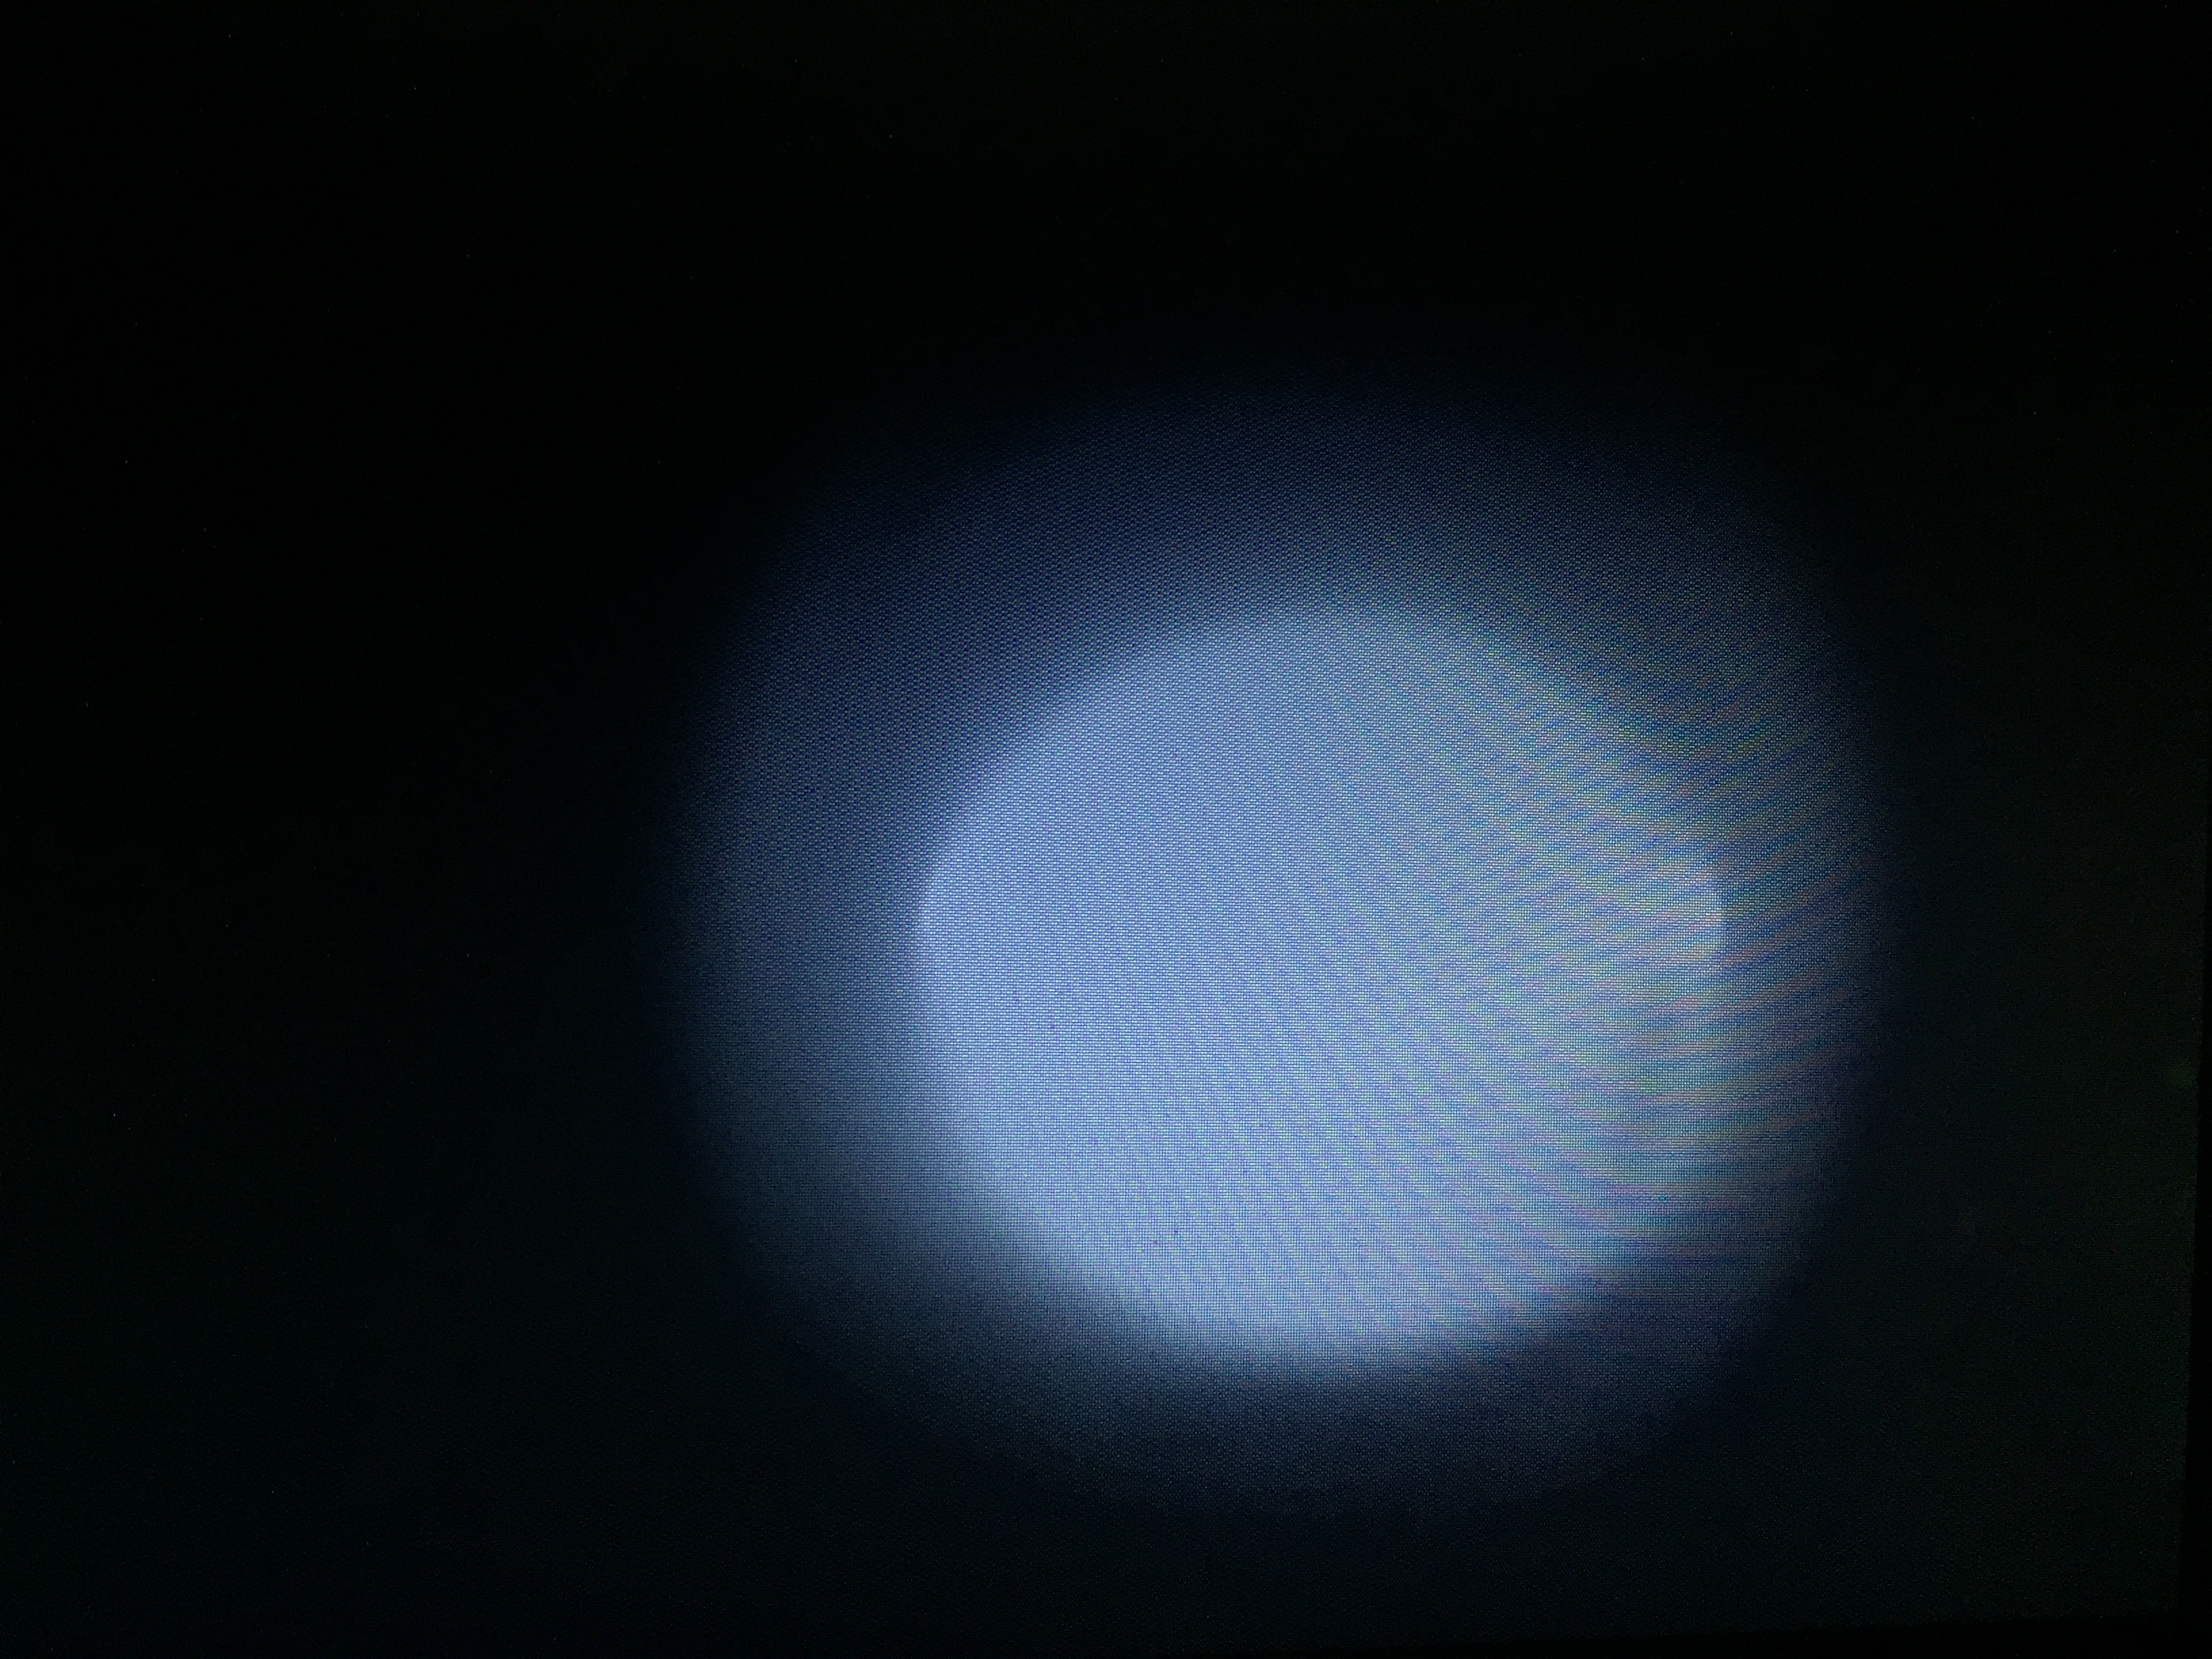
\includegraphics[height = 4cm]{pics/no_fluo.jpg}
    \caption{Cell hit by a wavelength outside of the absorption spectrum.}
    \label{fig:no_fluo}
  \end{subfigure}
  \begin{subfigure}{0.45\textwidth}
    \centering
    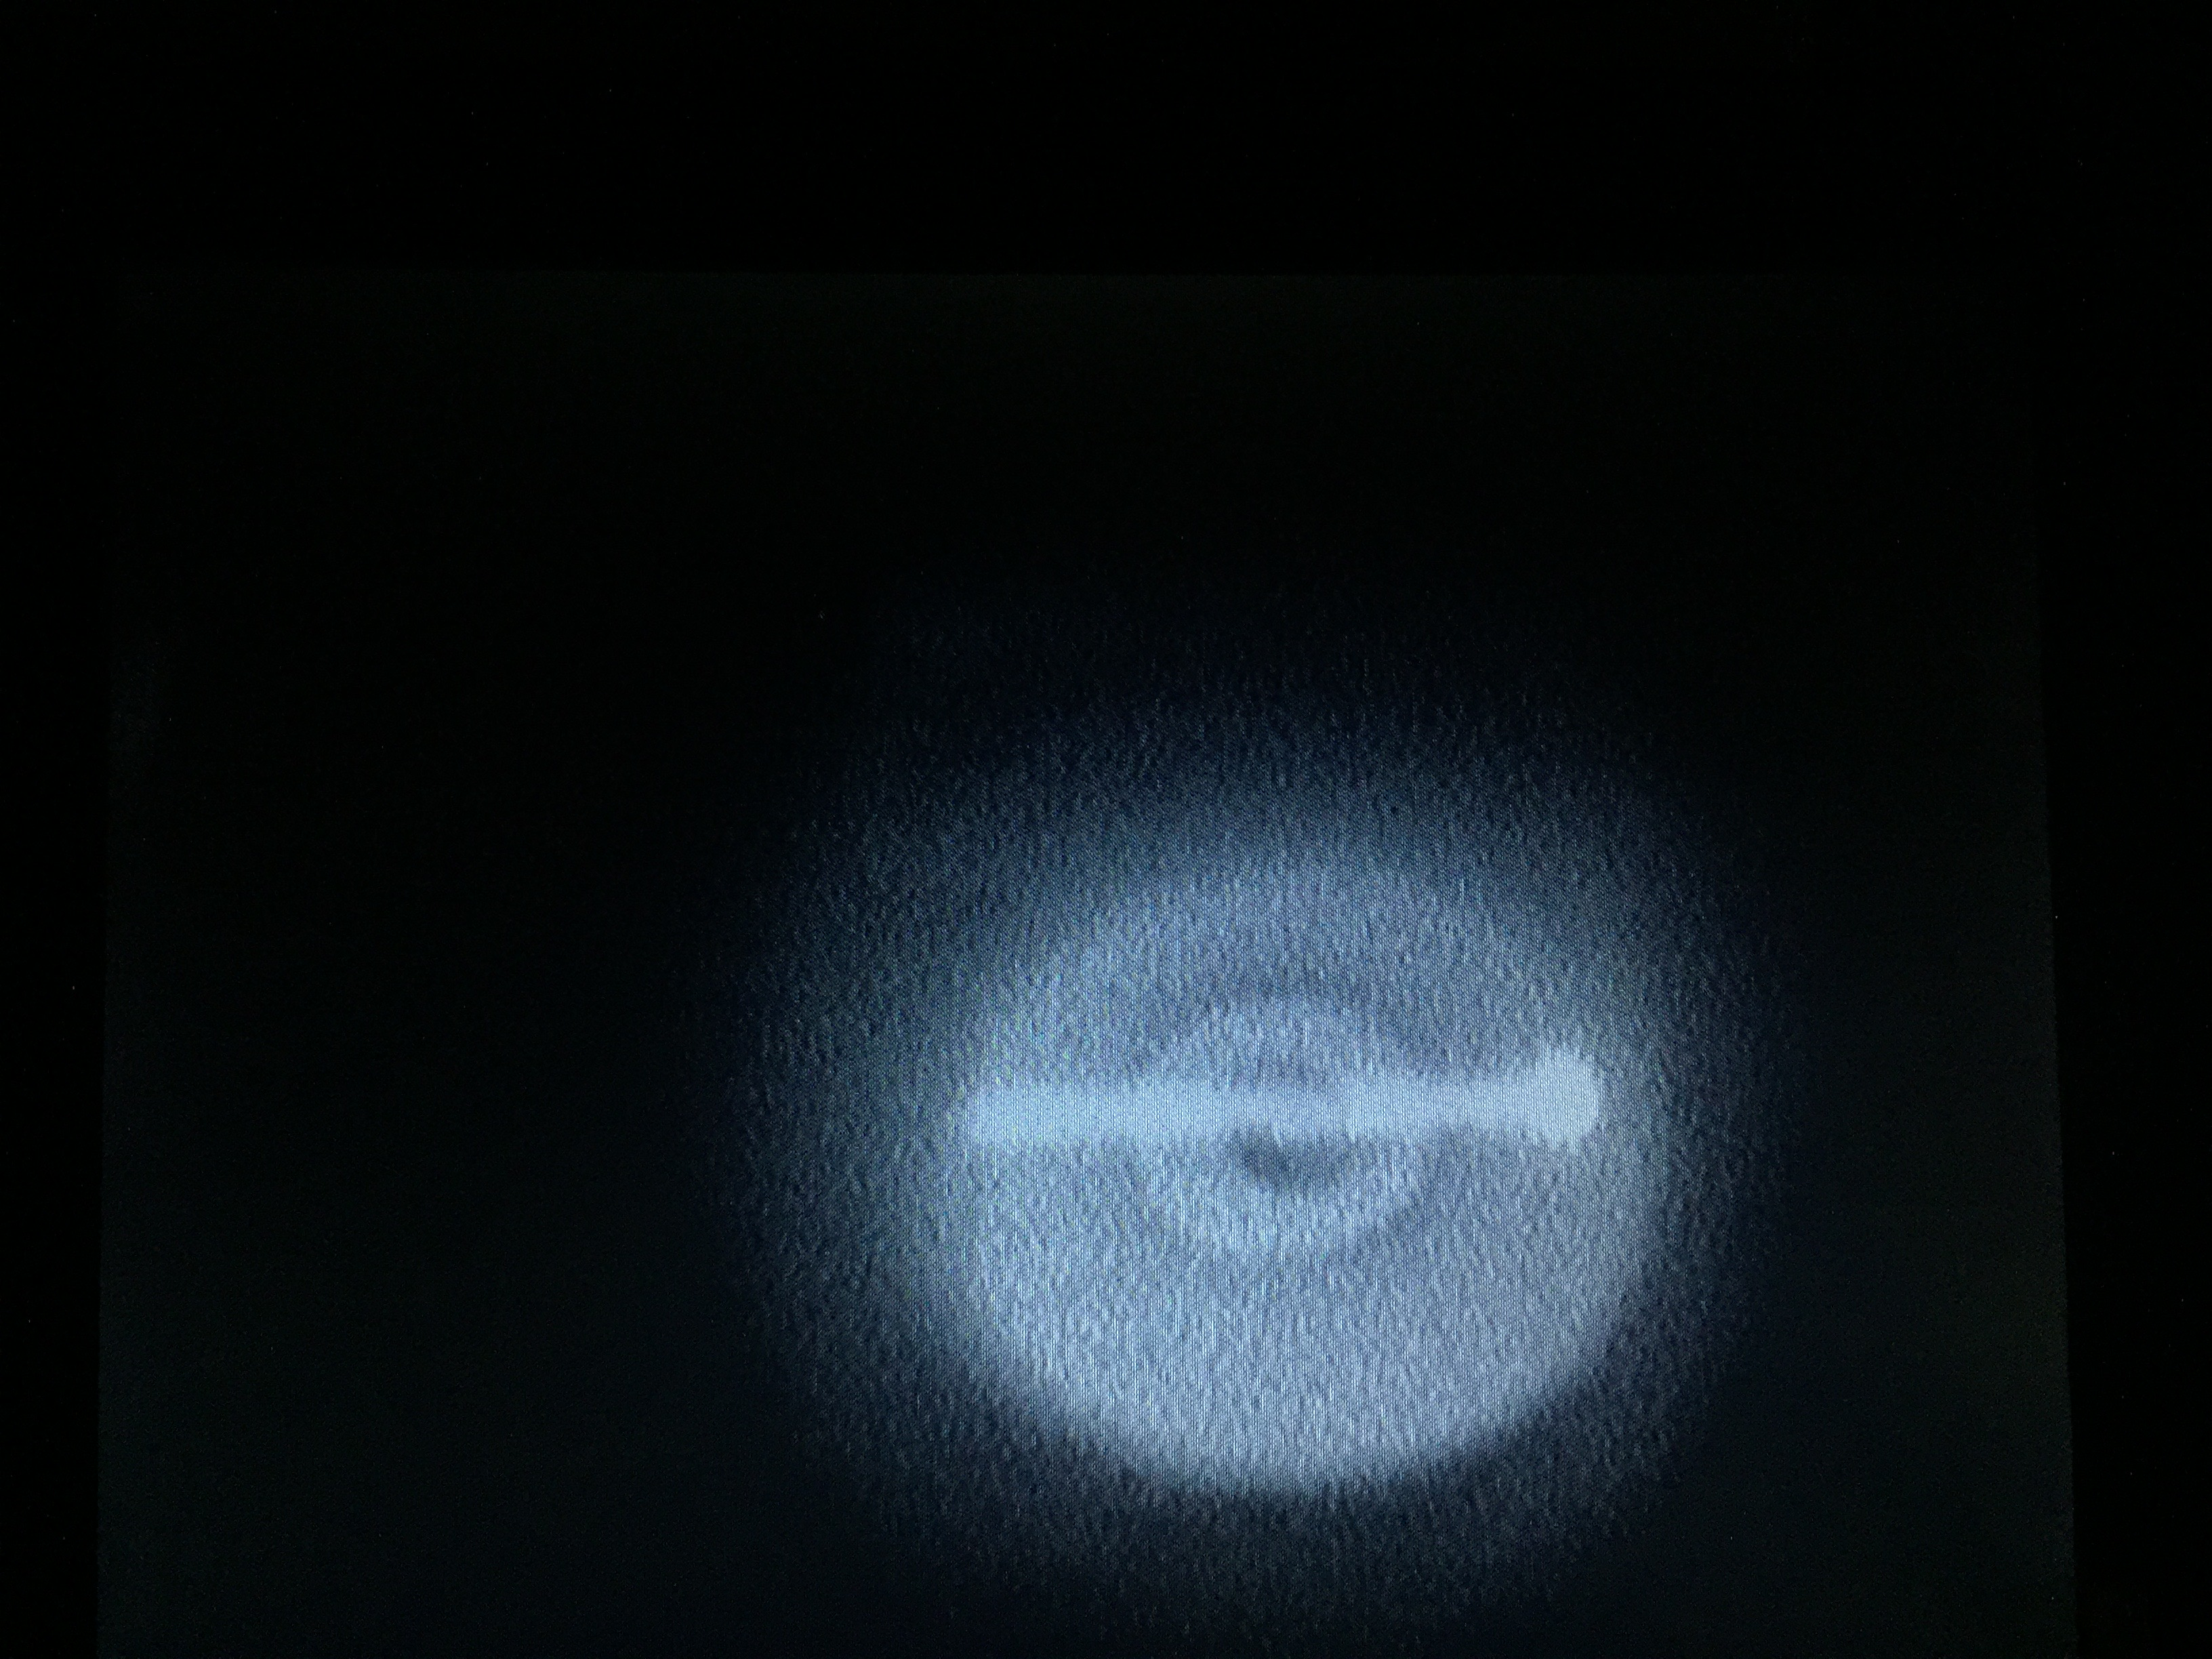
\includegraphics[height = 4cm]{pics/fluo.jpg}
    \caption{Cell hit by a wavelength inside of the absorption spectrum.}
    \label{fig:fluo}
  \end{subfigure}
  \caption{Pictures of the rubidiumcell enlightened by different wavelengths.}
  \label{fig:fluo_no_fluo}
\end{figure}

\subsection{The Absorption Spectrum of Rubidium}

Now that we obtained a laser with a fitting intensity and a wavelength near to the absorption spectrum the next step is to loop over a few different wavelengths to record the whole spectrum. To achieve this we connect a ramp generator to the piezo controller. This enlargens the piezoelectric stack which moves the gatter therefore vary the length of the external cavity and results in a periodically changing wavelength. In figure \ref{fig:triangle_with_absorption} the voltage applied to the piezo monitor and the signal of one photodiode after the cell is shown. The signal of the photodiode may be a bit wrong because at this part of the experiment the laser did not hit the diode completely.

\begin{figure}
  \centering
  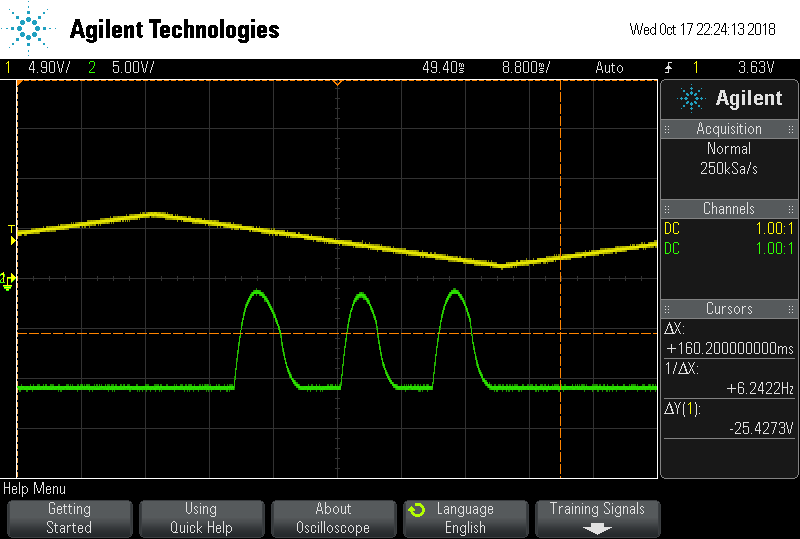
\includegraphics[height = 5cm]{pics/scope_199.png}
  \caption{Voltage on the piezoelectric stack and some absortion dips from one photodiode.}
  \label{fig:triangle_with_absorption}
\end{figure}

Now we connect the ramp generator besides its connection to the piezo controller also to the laser current. This allows a larger scan area without mode hops. With the right settings figure \ref{fig:dreieck_mit_absorption} is shown on the oscilloscope screen.
\begin{figure}
  \centering
  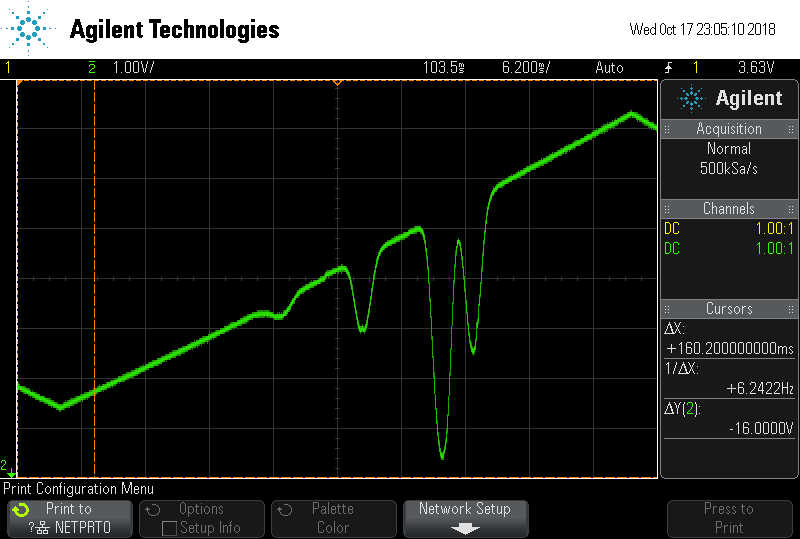
\includegraphics[height = 5cm]{pics/dreieck_mit_absorption.png}
  \caption{Signal of one photodiode with synchronized current and piezo controller.}
  \label{fig:dreieck_mit_absorption}
\end{figure}
To surpress the effect of the changing laser intensity we place a beam splitter in front of the cell which reflects one half of the laser beam to another photodiode. After this we can substract the signal of the laser which went through rubidium, from the laser signal which went directly into the second photodiode. By balancing the two signals with the controls on the subtraction controller a nice picture of the absorption spectrum can be achieved and is shown in figure \ref{fig:perfect_absorption}.
\begin{figure}
  \centering
  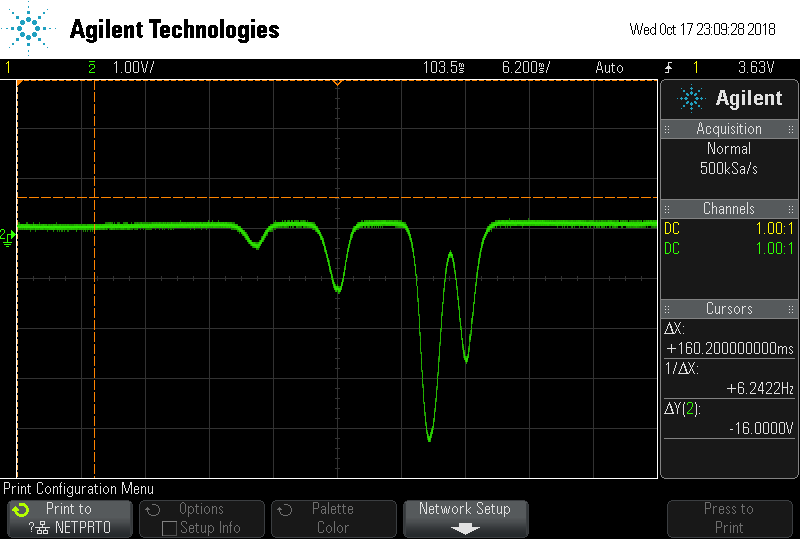
\includegraphics[height = 5cm]{pics/perfect_absorption.png}
  \caption{The recorded absorption spectrum of the two rubidium isotopes.}
  \label{fig:perfect_absorption}
\end{figure}

% \begin{figure}
%   \centering
%   \includegraphics{build/plotElement.pdf}
%   \caption{Plot.}
%   \label{fig:plot}
% \end{figure}
%
% Tabelle für copy and paste:
% \begin{table}[h]
%   \centering
%   \begin{tabular}{S S}
%     \toprule
%     {$k$} & {$U\:/\:\si{\milli\volt}$}\\
%     \midrule
%     1 & 637.2\\
%     3 & 212.4\\
%     5 & 127.4\\
%     7 & 91.03\\
%     9 & 70.8\\
%     \bottomrule
%   \end{tabular}
%   \caption{Amplituden Rechteckspannung.}
%   \label{tab:rechtampl}
% \end{table}

\section{Diskussion}
\label{sec:Diskussion}

\subsection{Messung einer Stromspannungskennlinie}

Die mit der Stromspannungskennlinie bestimmte Depletionsspannung lautet
\begin{align}
  U_\text{Dep,I(U)} = \SI{65.09}{\volt}
  \label{eqn:UdepI}
\end{align}
und liegt im Bereich der vom Hersteller genannten Depletionsspannung
\begin{align}
  U_\text{Dep,Hersteller} \approx \SI{60}{\volt} - \SI{80}{\volt}.
\end{align}
Jedoch ist an Abbildung \ref{fig:stromspannungskennlinie} erkennbar, dass
der Leckstrom erst bei deutlich höheren Vorspannung $> \SI{100}{\volt}$ sichtbar
linear mit der Spannung ansteigt, weshalb es sinnvoll ist, die Vorspannung in den
anschließenden Messreihen höher als \eqref{eqn:UdepI} einzustellen.

\subsection{Pedestal, Common Mode Shift und Noise}

Der bestimmte mittlere Pedestal liegt im Durchschnitt bei
\begin{align}
  \text{Pedestal}_\text{average} = 509.122 \pm 2.210 \, \text{ADC}
\end{align}
und damit am erwarteten Wert $\SI{500}{\text{ADC}}$.

Der Common Mode Shift ist in Abbildung \ref{fig:cms} als normiertes Histogramm dargestellt.
Die gaußförmige Verteilung durch den zentralen Grenzwertsatz ist zwar erkennbar, allerdings
mit sichtbaren statistischen Schwankungen. Das ist darauf zurückzuführen, dass lediglich
1000 Events für diese Messung aufgenommen wurden.

Der sich ergebende mittlere Noise liegt bei
\begin{align}
  \text{Noise}_\text{average} = 2.119 \pm 0.081 \, \text{ADC}.
  \label{eqn:noise}
\end{align}
und schwankt mit einem relativen Fehler von $\SI{3.8}{\percent}$ schwach für
jeden Streifen.

\subsection{Kalibrationsmessungen}

In Abbildung \ref{fig:kalibration} ist erkennbar, dass die Kalibrationskurven der Kanäle 20,40,60,80,100
für eine Vorspannung oberhalb der Depletionsspannung quasi alle aufeinander liegen. Das Polynom vierten Grades
nähert diese im Bereich $\text{charge} = [0,250000 \symup{e}]$ ausgezeichnet an, was ebenfalls in der
Abbildung ersichtlich ist.

Die Kalibrationskurve bei $\SI{0}{\volt}$ ist in Abbildung \ref{fig:kalibration2} mit den anderen Kurven
in einem großen Bereich (in dem die Diskrepanz der Messwerte am ehesten erkennbar ist) dargestellt.
An dieser Graphik ist erkennbar, dass das Einstellen der Depletionsspannung
eine wichtige Rolle spielt, da Signale bei der Umrechnung ansonsten um etwa $\SI{5}{\text{ADC}}$ abweichen, was
beispielsweise doppelt so viel wie der berechneten durchschnittliche Noise \eqref{eqn:noise} ist.

\subsection{Vermessung der Streifensensoren mittels eines Lasers}

Aus Abbildung \ref{fig:pitch} ist entnehmbar, dass der Laser über die Kanäle 91 und 92 bewegt wurde.
Die berechnete pitch liegt bei
\begin{align}
  \text{pitch}_{92-91} = \SI{161.69}{\micro\meter}
\end{align}
und weicht damit relativ gering um $\SI{1}{\percent}$ von der vom Hersteller genannten pitch
\begin{align}
  \text{pitch}_\text{Hersteller} = \SI{160}{\micro\meter}
\end{align}
ab. Der Sitz der Kathode ist zur Vermessung ionisierender Strahlung irrelevant, da diese Strahlung
kaum von der Metallisierung reflektiert wird. Beim Laserstrahl wird genau die Tatsache, dass das
Licht reflektiert wird, zur Vermessung des Streifensensors ausgenutzt und zwar erfolgreich,
wie an der geringen Abweichung erkennbar ist.

\subsection{Charge Collection Efficiency Messungen mit dem Laser}

Die mit der Charge Collection Efficiency Messung mit dem Laser berechnete Depletionsspannung
\begin{align}
  U_\text{dep,ccel} = \SI{110(5)}{\volt}
\end{align}
ist wesentlich größer als die mit der Stromspannungskennlinie bestimmte Depletionsspannung
\begin{align}
  U_\text{Dep,I(U)} = \SI{65.09}{\volt}.
\end{align}
Das ist darauf zurückzuführen, dass die Leckstrommessung zwar ein guter Indikator für das Erreichen der
Depletionsspannung ist, aber die Vorspannung, die tatsächlich für die Signalmessung eingestellt werden sollte,
größer ist. Der Grund dafür liegt darin, dass beim Erreichen der Depletionsspannung das äußere elektrische Feld noch nicht
ausreichend stark ist, um jedes entstehende Elektron-Loch-Paar an der Rekombination zu hindern. Der Leckstrom steigt aus diesem
Grund auch weiter an, wenn die Spannung über die Depletionsspannung hinausgeht: ein immer größerer Anteil der durch
thermische Anregung erzeugten Elektron-Loch-Paaren erreicht die Pole und rekombiniert nicht.

\subsection{Charge Collection Efficiency Messungen mit der Quelle}

Die mit der Charge Collection Efficiency Messungen mit der Quelle berechnete Depletionsspannung
\begin{align}
  U_\text{depl,cceq} = \SI{120(5)}{\volt}
\end{align}
weicht mit $\SI{9}{\percent}$ leicht von der Messung mit dem Laser ab. Was außerdem in Abbildung
\ref{fig:cceq} heraussticht, ist, dass das Plateau eine leichte Steigung besitzt. Das ist darauf zurückzuführen, dass
das Elektron aus dem radioaktiven $\beta$-Zerfall im Gegensatz zu den Photonen aus dem Laser durch das
elektrische Feld im Detektor leicht abgebremst wird. Wird die Spannung erhöht, so steigt die elektrische Feldstärke
und das Elektron hält sich länger im Detektor auf, sodass sich die Anzahl an Stoßprozessen erhöht und die Energiedeposition steigt.

\subsection{Großer Quellenscan}


\printbibliography

\appendix
\section{Kopie der Originaldaten}

\begin{figure}[h]
  \centering
  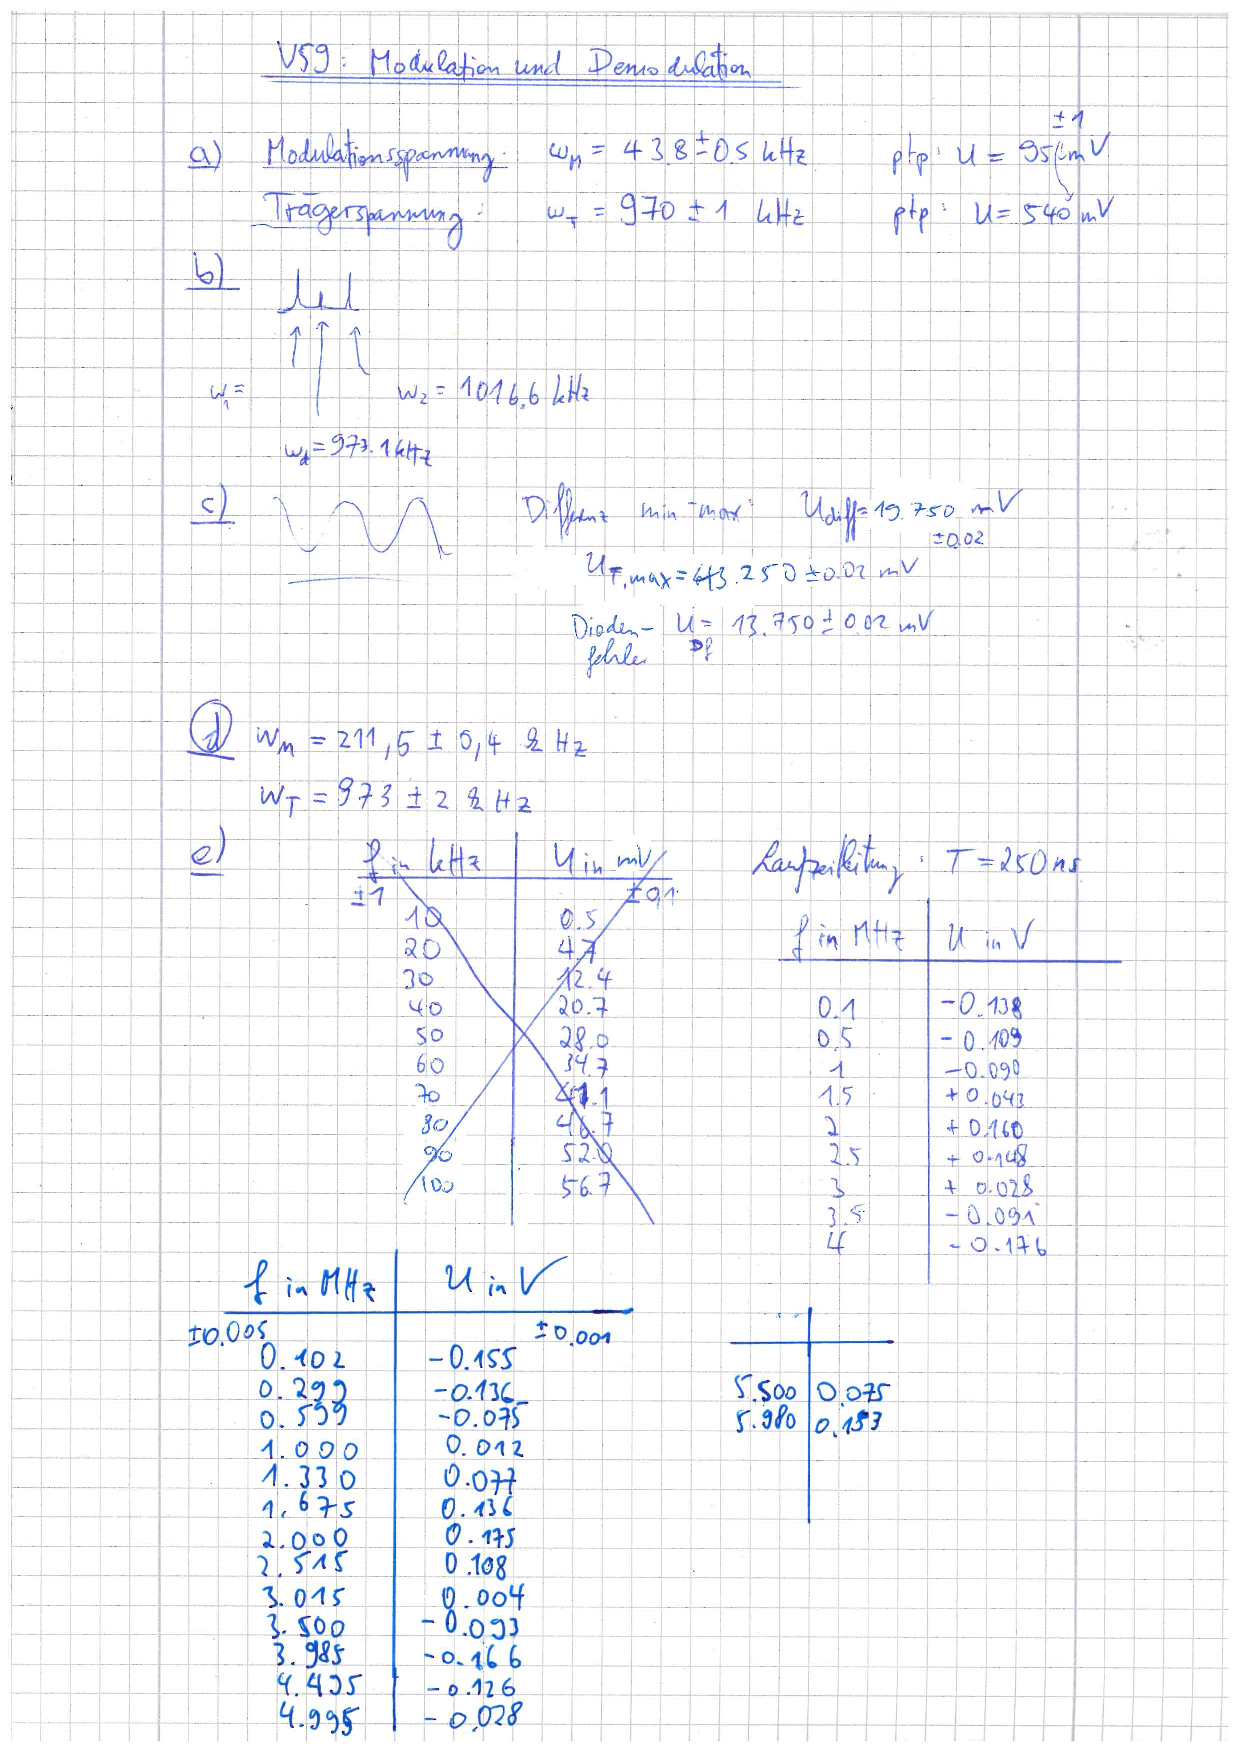
\includegraphics[width=.9\textwidth]{Messwerte.pdf}
  \caption{Kopie der Messdaten.}
  \label{fig:hnachSchwingkreis}
\end{figure}

\end{document}
